\chapter{Application}\label{chap:application}

\newcommand{\download}{Download\xspace}
\newcommand{\live}{Live\xspace}
\newcommand{\serviceprovisioning}{Provisioning\xspace}
\newcommand{\streaming}{Streaming\xspace}

While the previous chapter focussed on the network and the impact of applications, vendors, and users thereon, this chapter shifts focus on the applications.
The Internet supports a multitude of different applications, including video streaming services, online gaming, file storage services, cloud office solutions, and uncountable more.
In this chapter, we focus on two of the most prominent application types: Video streaming and file storage, chosen due to their impact on global traffic and frequency of use.
In contrast to applications of earlier generations, todays services are not standardised or under control by network operators but rather the result of free enterprise and enterpreneurship.
While in the last chapter we were able to rely on standard documents to model the systems under study, this option is no longer available when considering applications.
Thus, we have to perform measurements or rely on studies of other researchers in order to obtain knowledge of both the systems under study as well as the related stakeholders.

Similar to \refchap{chap:network}, we identify a set of involved stakeholders and their respective key performance indicators and derive corrosponding metrics.
First, we consider the application provider. 
In the case of the video streaming scenario, this role is realised by the video provider.
We consider the video provider to be interrested in two performance indicators: 
\begin{enumerate*}
\item user satisfactiom, realised by a \gls{QoE} metric,
\item cost reduction in compute and network infrastructure, realised by the amount of traffic transmitted to a user about to abort playback.
\end{enumerate*}
In the case of the file synchronisation scenario, we consider the application operator to be interrested in user satisfaction, again realised by as \gls{QoE} metric, the mean time to synchronisation.
Wasted traffic is not of concern in this scenario, as file synchronisations are usually not aborted.
Second, we consider the network operators.
As in the last chapter, they are interested in reducing stress on the network infrastructure.
We measure this key performance indicator by considering the metric 
%cite?

Overview of Stakeholders

Current best practices

The contribution of this chapter is threefold:
\begin{enumerate*}
\item lte video
\item qoe user behaviour
\item cloud file synchronization
\end{enumerate*}

The content from this chapter has been published in \cite{Schwartz2013b, Hossfeld2015, Schwartz2014a}.
\refsec{sec:application:background} we discuss the current state of the art regarding video transmission mechanisms and \gls{QoE} studies.
Then, in \refsec{sec:application:lte_video} we discuss tradeoffs between different video transmission mechanisms, regarding the considered metrics.
In \refsec{sec:application:qoe_user_behaviour} we study the impact of user preferences on the \gls{QoE} experienced during video streaming.
Finally, in \refsec{sec:application:cloud_file_synchronisation} we consider the impact of different file synchronisation scheduling algorithms on the relevant stakeholders.

\section{Background and Related Work}\label{sec:network:background}

\subsection{\headershortacr{UMTS} Networks and the \headershortacr{RRC} Protocol}\label{sec:network:background:umts_rrc}
A \gls{3G} \gls{UMTS} mobile network consists of three main components, which are depicted in \reffig{fig:network:background:mobile_network_overview}: The \gls{UE}, the \gls{RAN}, and the \gls{CN}.
The \gls{RAN} is used to establish connectivity between the \gls{UE} and the \gls{CN}, which in turn can establish connectivity to the Internet, if required.

\begin{figure}
	\centering
	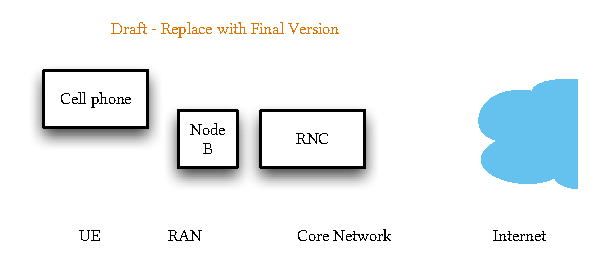
\includegraphics{network/background/figures/mobile_network_overview}
	\caption{Overview of Mobile Network}
	\label{fig:network:background:mobile_network_overview}
\end{figure}

\gls{UE} consists of devices used by end users, i.e. smartphones, tablets or data card enabled notebooks, but can also include \gls{M2M} devices.
The \gls{RAN} is, amongst other tasks, responsible for \gls{RRC}, packet scheduling and handover control.
It includes network entities such as the \gls{NodeB} and the \gls{RNC}.
The \gls{CN} provides the backbone network of the \gls{UMTS} network and provides connectivity to the Internet and the \gls{PSTN}.
Furthermore, functionality such as billing, authentication and location management is provided by the \gls{CN}.

In UMTS networks, the radio resources in the RAN between base station and UE are controlled and managed by the \gls{RRC} protocol~\cite{3GPP_RRC_Spec}.
The protocol offers services such as broadcast of network information, maintenance of a connection between the \gls{UE} and \gls{RAN}, establishment of point-to-point radio bearers for data transmission, \gls{QoS} control, and reporting and cell selection management.
The protocol is divided into different parts: services for upper layers, communication with lower layers, protocol states, \gls{RRC} procedures, and error control.
In particular, \gls{RRC} also participates in the co-ordination of other resource management operations such as channel measurements and handovers.
All \gls{RRC} procedures rely on protocol states which are defined to trigger action should be applied and which information must be signaled. 
The state are defined per \gls{UE} and for the connection between the \gls{UE} and the \gls{NodeB} station.
Typically there are five \gls{RRC} states characterizing a connection between \gls{UE} and \gls{NodeB}: \gls{idle}, \gls{URAPCH}, \gls{CELLPCH}, \gls{DCH}, and \gls{FACH}.
Whether a specific \gls{RRC} state is used in a specific mobile network depends on the configuration of the network by the provider.
In the following we concentrate on the most commonly observed~\cite{Qian2010} \gls{RRC} states \gls{idle}, \gls{DCH}, and \gls{FACH}.

\subsection{Measurements of \headershortacr{RRC} Parameters and Optimisation of Resource Consumption}\label{sec:network:background:measurement_optimisation}

\subsection{Smartphone Energy Consumption and \headershortacr{QoE}}\label{sec:network:background:energy_consumption_qoe}

\section{Trade-Offs for Multiple Stakeholders in LTE}\label{sec:application:lte_video}

\newcommand{\bandwidth}{\ensuremath{b_W}\xspace}
\newcommand{\bitrate}{\ensuremath{b_R}\xspace}
\newcommand{\timeplayedback}{\ensuremath{t_p}}

\newcommand{\streamingstart}{\ensuremath{\sigma}\xspace}
\newcommand{\bufferlower}{\ensuremath{\theta}\xspace}
\newcommand{\buffersize}{\ensuremath{\Theta}\xspace}

\newcommand{\ton}{\(T_{\texttt{ON}}\)\xspace}
\newcommand{\tdrxinactivity}{\(T_{\texttt{I}}\)\xspace}

\newcommand{\shortdrx}{\texttt{Short DRX}\xspace}
\newcommand{\tshortdrx}{\(T_{\texttt{S}}\)\xspace}
\newcommand{\longdrx}{\texttt{Long DRX}\xspace}
\newcommand{\tlongdrx}{\(T_{\texttt{L}}\)\xspace}
\newcommand{\rrcconnected}{\texttt{RRC Connected}\xspace}
\newcommand{\tidle}{\(T_{\texttt{Idle}}\)\xspace}
\newcommand{\tonidle}{\(T^{\texttt{Idle}}_{\texttt{ON}}\)\xspace}
\newcommand{\rrcidle}{\texttt{RRC Idle}\xspace}
\newcommand{\tdrxidle}{\(T^{\texttt{Idle}}_{\texttt{\gls{DRX}}}\)\xspace}
\newcommand{\promotiondelay}{\(D_P\)\xspace}

\newcommand{\bandwidthdown}{b_d\xspace}
\newcommand{\timedownloaded}{\ensuremath{t_d}}

\newcommand{\power}{P\xspace}
\newcommand{\energyconsumption}{\ensuremath{E}\xspace}
\newcommand{\connectioncount}{\ensuremath{C}\xspace}

\newcommand{\factordown}{\ensuremath{\alpha}\xspace}
\newcommand{\powerbaseline}{\ensuremath{\beta}\xspace}

\newcommand{\userabortrv}{\ensuremath{A}\xspace}
\newcommand{\userabortpdf}{\ensuremath{a}\xspace}
\newcommand{\meanwastedtraffic}{\ensuremath{W}\xspace}

\newcommand{\timeunwatched}{\ensuremath{t_u}}
\newcommand{\videolength}{l\xspace}

The consumption of video content in a mobile scenario is one of the premier use cases for the \gls{LTE} mobile communication technology.
While the use of \gls{LTE} affords sufficient bandwidth to enable video playback in high definition, it also introduces new challenges for all stakeholders.
Similarly to the applications discussed in \refchap{chap:network}, signalling traffic induced by the video transmission may pose a challenge for mobile network operators, and power drain remains an open issue for hardware vendors.
Additionally, mobile playback can cause new problems for video providers.
Users watching video on the go may be prone to higher rates of interrupted video playback, either due to insufficient network coverage or social interactions.
If the video transmission mechanism has transmitted too much video content in advance, this transmitted data is ``wasted'', from the perspective of the video provider, as it consumed both network and computation resources but resulted in no benefit for the customer.

First, in \refsec{sec:application:lte_video:system_model} we present models for both video playback and the mobile network.
Then, in \refsec{sec:application:lte_video:numerical_evaluation} we perform a simulative study using the proposed model in order to evaluate the performance of the studied video transmission mechanisms.

\subsection{System Model for File Synchronisation using Dropbox}\label{sec:application:cloud_file_synchronisation:system_model}
This section first provides a general overview over the Dropbox service architecture and introduces the considered use case.
Then, we propose the cloud storage model and metrics used in this analysis.
Finally, we discuss a set of scheduling mechanisms used to start the file synchronisation process.

The authors of~\cite{Drago2012} provide a first study of the \dropbox architecture, which is schematically depicted in \reffig{fig:application:cloud_file_synchronisation:system_model:dropbox_architecture} and used as a basis for the model under study in the remainder of this section.

\begin{figure}
  \centering
  \includegraphics[width=\columnwidth]{application/cloud_file_synchronization/system_model/figures/dropbox_architecture}
  \caption{\dropbox file storage and retrieval process.}
  \label{fig:application:cloud_file_synchronisation:system_model:dropbox_architecture}
\end{figure}

The \dropbox infrastructure consists of two main components:
\begin{enumerate*}
\item a storage cloud based on Amazon's Elastic Compute Cloud and Simple Storage Service, and
\item control servers directly maintained by \dropbox Inc.
\end{enumerate*}
The control servers store meta information about the current state of the files in the \dropbox folders and trigger synchronisation processes on the clients.

A file synchronisation can basically be described in five steps.
As soon as the new file is added to the \dropbox folder of the uploading client, a preprocessing step is triggered and the meta information for the file are generated, respectively updated.
This information is then synchronised with the control servers~(1) and the file itself is uploaded to the storage cloud~(2).
After the file has completely been transferred to the storage cloud, all connected clients are notified about the update~(3) and start downloading the new file~(4).

\subsubsection*{Use Case: Photo Uploading}\label{sec:application:cloud_file_synchronisation:use_case}
In this section we consider the synchronisation of images from a digital camera to a mobile \gls{UE} via a cloud storage provider.
Real world examples of this scenario are, e.g., taking photos of a live event and transferring them to a picture agency, or shooting private holiday images.

The user took a finite set of pictures with a wearable device like Google Glass or a smart camera, e.g. a Nikon Coolpix S800c or SAMSUNG CL80.
The camera is then connected via a \gls{PAN} with a mobile \gls{UE}, for example a laptop with a data card or a smartphone, to store the images on the mobile device.
The \gls{UE} uses broadband wireless Internet access technology and runs software provided by the cloud storage provider in order to synchronise the images with the cloud storage.
Finally, the scenario includes a remote client, which is connected using a wire line connection and downloads the images from the cloud.

For the evaluation we consider a specific realisation of the use case described above.
For the role of the cloud storage provider we consider \dropbox, Bluetooth is used as the technology for establishing the \gls{PAN}, and \gls{LTE} is used as the wireless broadband access technology.

In the considered scenario the interests of two stakeholders are impacted.
The first stakeholder, the end user, has two contradicting requirements on the system.
On the one hand, the images should be synchronised as fast as possible.
This requires a fast and permanent Internet connection of the \gls{UE}, which in turn is very power intensive.
On the other hand, the power drain of the mobile device should be minimised to enable a long battery life time.
The second stakeholder, the mobile network provider, wants to minimise the signalisation overhead in the network~\cite{NSN2011, Huawei2011} caused by short time connections.
Here, an optimisation problem arises to find a practical solution for all three requirements.
In order to analyse this problem, we use a simulation model of the file synchronisation process, which is described in the following.

\subsubsection*{Cloud Storage Model and Performance Metrics}\label{sec:application:cloud_file_synchronisation:system_model:model_metrics}
The proposed simulation model is schematically depicted in \reffig{fig:application:cloud_file_synchronisation:system_model:model_metrics:model} and based on the findings of~\cite{Drago2012} described in~\refsec{sec:application:background}.

\begin{figure}
\centering
\includegraphics[width=\columnwidth]{application/cloud_file_synchronization/system_model/figures/model}
\caption{Considered synchronisation process model.}
\label{fig:application:cloud_file_synchronisation:system_model:model_metrics:model}
\end{figure}

We assume that the user has taken pictures of varying file size distributed with \imageFileSize.
These pictures are transferred from the camera to the mobile device using the \gls{PAN} with a constant bandwidth~\panTransferRate.
Due to the limited bandwidth \panTransferRate of the \gls{PAN} device, the inter-arrival times of images at the \dropbox shared folder of the mobile device can be calculated by \(\interarrivaltime = \frac{\imageFileSize}{\panTransferRate}\).

As soon as the image is fully copied to the \dropbox folder, the generation of the meta data introduces a preprocessing delay, which we refer to as client preparation time~\clientpreparationtime.
To evaluate different strategies optimising the overall waiting time, power drain, and signalisation traffic we include a scheduling component.
This component implements different algorithms, which trigger sending the images currently held available in the scheduling component to the component responsible for transmission.

Next, we consider the \gls{LTE} \gls{UE} used for image upload.
Due to the specification of the \gls{LTE} standard \cite{3GPP_RRC_Spec}, the upload component can, at any point in time, either be connected to the mobile network or disconnected.
If the \gls{UE} is currently disconnected, and a new image for upload arrives, the connection process is triggered and completed after a startup delay \(\startupDelay = \SI{0.26}{\second}\).
Once the \gls{UE} is connected, arriving images are transmitted in order.
The transmission, i.e. service time, of an image depends on the size of the image currently being uploaded as well as the upload bandwidth \uploadbandwidth.
As only one image is transferred at once, waiting images are stored in a queue of infinite size.
If the \gls{UE} is idle for more than \(\idleThreshold = \SI{11.576}{\second}\), the device disconnects from the network.

After the image has been successfully uploaded to the storage servers, a server side preprocessing phase starts, before the file transfer to the downloading client starts.
This server side preprocessing again introduces an additional delay, the server preparation time~\serverpreparationtime, in the synchronisation process.
Finally, the image is downloaded by the wire line client.
Again, the duration is calculated based on the size of the image and the available download bandwidth~\downloadbandwidth.

Next, we discuss the metrics used to evaluate the performance of the scheduling algorithms under consideration.
First, we consider the mean synchronisation time \sojournTime, i.e., the time between the generation of images and the completion of the download.
This metric accounts for the desire of end users to synchronise images in a short amount of time.
Secondly, we study the relative amount of time the \gls{UE} is disconnected \relativeDisconnectedTime.
As the \gls{UE} consumes more power in the connected state, the user is generally interested in scheduling mechanisms which ensure that the device is only connected if required \cite{Ickin2012}.
This measure also enables a more general evaluation than the actually consumed power, as the concrete power drain differs significantly for each device.
Finally, we evaluate the number of transitions~\connectionCount between the connected and disconnected states.
As discussed in \refsec{chap:network}, frequent state transitions stress the network due to increased signalling.
Thus, scheduling algorithms with a small number of transitions would be favoured by network operators.

\subsubsection*{Considered Scheduling Algorithms}\label{sec:application:cloud_file_synchronisation:system_model:algorithms}
We use different scheduling strategies in our model to control the uploading of the files from the mobile client.
These mechanisms in turn affect the synchronisation time, the power drain, and the generated signalling traffic.

The most basic strategy of handing the upload is to immediately send new files, as soon as the meta data is generated.
We refer to this as the \algoimmediate strategy and will use this as base line for all comparisons in the evaluations.
The other two strategies considered are based on a temporal, respectively a size threshold.
Using the \algointerval scheduling, the client checks periodically, according to an interval \thresholdInterval, if new files have been marked for synchronisation.
If new files are present, they are synchronised to \dropbox.
Files which could not be sent within the current interval will automatically be added to the file batch for the next interval.
The last scheduling mechanisms uses a threshold \thresholdSize based on the overall \algosize of the images not yet synchronised.
If the threshold is crossed, an upload is triggered.

\subsection{Numerical Evaluation}\label{sec:application:lte_video:numerical_evaluation}

In this section we study the metrics introduced in \refsec{sec:application:lte_video:system_model:model_assumptions:metrics} on the different transmission mechanisms.

First, we study the impact of the considered transmission mechanisms on the energy consumption and the wasted traffic. 
Then, in \refsec{sec:application:lte_video:connection_count} we consider the impact of the connection count for the \streaming mechanisms and varying values of the parameters \emph{stop threshold} \bufferlower and \emph{threshold size} \buffersize in more detail.

We consider a video of \(\videolength=\SI{1600}{\second}\) length which is viewed on a \gls{UE} with \gls{LTE} access.
The median of available downlink throughput in current \gls{LTE} networks is \(\bandwidth = \SI{12.74}{\mega\bit\per\second}\) \cite{Huang2012}.
A wide set of video bitrates between \SIlist{1;50}{\mega\bit\per\second} is in use~\cite{YouTube2013}.
In order to prevent stalling, we consider bitrates between \SIrange{1}{10}{\mega\bit\per\second}, staying below the available network bandwidth.
For the \streaming mechanism, a stop threshold of \(\bufferlower = \SI{4}{\second}\) and a threshold size of \(\buffersize = \SI{32}{\second}\) were selected.
Furthermore, we specify a prebuffering duration of \(\streamingstart = \SI{5}{\second}\).

We conduct our study using deterministic discrete event simulation which uses no random variables.
The wasted traffic is obtained analytically using the abort behaviour model.
Thus, all results are exact under the previously stated assumptions.

\subsubsection*{Energy Consumption}\label{sec:application:lte_video:numerical_evaluation:energy_consumption}
First, we study the influence of both video bitrate as well as the selected download mechanism on energy consumption in \reffig{fig:application:lte_video:numerical_evaluation:energy_consumption:bitrate2energy}.
\begin{figure}
  \centering
  \includegraphics{application/lte_video/numerical_evaluation/figures/bitrate2energy}
  \caption{Influence of bitrate and download mechanism on energy consumption}
  \label{fig:application:lte_video:numerical_evaluation:energy_consumption:bitrate2energy}
\end{figure}

We consider the \download mechanism and observe that it consumes the least amount of energy.
Here the video is downloaded with full bandwidth, as seen in \reffig{fig:application:lte_video:system_model:video_model}, resulting in a very short energy intensive download phase and a longer energy un-intensive playback phase.
For the \live mechanism we observe the opposite, i.e. the highest energy consumption for all bandwidths.
If this mechanism is used, the used bandwidth equals the video bitrate.
Thus, the download requires the same amount of time as the playback, resulting in the highest possible energy consumption.
The \serviceprovisioning method uses a higher bandwidth, thus reducing the overall download time.
This reduced download time decreases the energy consumption when compared to the \live mechanism, even though the bandwidth used for downloading is increased to \SI{120}{\percent}.
For the \streaming mechanism we observe an energy consumption slightly higher than the \download mechanism.
As the bitrate of the video increases, the energy consumption increases as well.
This is due to the fact that a higher video bitrates require larger downloads.
For video bitrates approaching the available bandwidth the \streaming mechanism degenerates to the \live mechanism, as no prebuffering is possible.
We conclude that the \download and \streaming mechanisms outperform \live and \serviceprovisioning with regard to energy consumption.

\subsubsection*{Wasted Traffic}\label{sec:application:lte_video:numerical_evaluation:wasted_traffic}
Next, we consider the wasted traffic as a metric of the transmission mechanism quality.
If a user completely watches a video, no traffic is wasted.
Thus, we consider only the cases where a user stops the playback before the video is finished.
\begin{figure}
  \centering
  \includegraphics{application/lte_video/numerical_evaluation/figures/bitrate2lostData}
  \caption{Influence of bitrate, download mechanism and user model on wasted traffic}
  \label{fig:application:lte_video:numerical_evaluation:energy_consumption:bitrate2lostData}
\end{figure}
In \reffig{fig:application:lte_video:numerical_evaluation:energy_consumption:bitrate2lostData} we study the wasted traffic for different video bitrates.
We consider the different transmission mechanisms introduced in \refsec{fig:application:lte_video:system_model:video_model} as well as the previously introduced user models.
We observe that the choice of user model has no significant impact on the wasted traffic.
For the \download mechanism, the amount of wasted traffic increases up to a video bitrate of \SI{6}{\mega\bit\per\second}, then the wasted traffic decreases as only video data which has been prebuffered can be lost if the user aborts the video.
As we assume a available bandwidth of \SI{12.74}{\mega\bit\per\second}, the bandwidth available for prebuffering decreases as the bitrate increases, resulting in lower amounts of wasted traffic for high video bitrates.
For the \live mechanism, we see that the wasted traffic for all user models is very low, but wasted traffic exists.
This is due to the traffic already sent by the server while the \gls{UE} is still waiting for promotion from \rrcidle to \rrcconnected, i.e. a short prebuffering phase exists.
As the bandwidth increases with the video bitrate, the wasted traffic increases as well.
Next, we consider the \serviceprovisioning approach and see an increase of wasted traffic as the video bitrate increases, due to the fact that the bandwidth used for continuous download is a factor of the video bitrate.
A higher video bitrate results in the download of the video being completed earlier, which leads to more wasted traffic.
Similar results can be seen for the \streaming mechanism, which results in more wasted traffic than the \live mechanism, but significantly less traffic than the \serviceprovisioning mechanism.
This is due to the fact that if the user aborts, at least the amount of video given by the \emph{stop threshold} \bufferlower and at most the complete buffer, given by the \emph{stop threshold} and the \emph{threshold size} are lost.
We have observed that the choice of user model results in no qualitative changes in wasted traffic.
As we have seen, the \download and \streaming mechanisms provide best results with regard to energy consumption.
However with regard to wasted traffic, the \live and \streaming mechanisms are most suited.
Thus, the \streaming mechanism seems to be a good compromise.
The network operator can select a tradeoff between energy consumption and wasted traffic as discussed in the next section.
From now on, we only consider the uniformly distributed user model.

\subsubsection*{Connection Count}\label{sec:application:lte_video:connection_count}
The \gls{ISP} is interested in reducing the number of connections occurring during video transmission.
Thus, we quantify the impact of the selected video transmission mechanism on the connection count, which directly correlates with the occurring signalling.
\begin{figure}
  \centering
  \includegraphics{application/lte_video/numerical_evaluation/figures/bitrate2connections}
  \caption{Influence of bitrate and download mechanism on connection counts}
  \label{fig:application:lte_video:numerical_evaluation:energy_consumption:bitrate2connections}
\end{figure}

In \reffig{fig:application:lte_video:numerical_evaluation:energy_consumption:bitrate2connections} we study the impact of the different transmission mechanisms on the number of connections per transmission and thus the amount of generated signalling.
We observe that for the transmission mechanisms download, live, provisioning the number of connections is constantly one, independent of the selected bitrate \bitrate.
This is due to the fact that in these transmission mechanisms the video is transmitted in one chunk.
For streaming, the number of connections decreases as the video bitrate increases.
Here, a connection occurs each time the buffer is refilled.
For larger bitrates, refilling the buffer requires a longer transmission.
As the maximum time of video transmission is upper bounded by the video length, longer buffering phases result in a smaller total amount of buffering phases and thus in less connections per video transmission.

\begin{figure}
  \centering
  \includegraphics{application/lte_video/numerical_evaluation/figures/bitrate2connections_parameters}
  \caption{Influence of bitrate and selected parameters on connection counts for the streaming mechanism}
  \label{fig:application:lte_video:numerical_evaluation:energy_consumption:bitrate2connections_parameters}
\end{figure}

Next, we consider the impact of the lower buffer threshold \bufferlower and buffer size \buffersize on the number of connections \connectioncount caused by the \streaming mechanism.
In \reffig{fig:application:lte_video:numerical_evaluation:energy_consumption:bitrate2connections_parameters} we observe that while the buffer size has a significant impact on the number of connections during a video transmission, the lower buffer threshold has almost no impact.
For buffer sizes of \SIrange{4}{8}{\second}, no signalling occurs.
This is due to the fact that, as discussed in \refsec{sec:application:lte_video:system_model:lte_network_model}, the connection timeout in \gls{UE} is configured as \SI{11.576}{\second}.
Thus, for this low buffer sizes the \gls{UE} does not disconnect from the network.
Furthermore, we observe that as the buffer size increases, the number of connections decreases.
Refilling larger buffers requires, similar to larger bitrates, longer transmission times.
Thus, due to the total upper bound on the transmission time, less download phases can occur during the transmission.
\subsection{Tradeoff Considerations for Participating Stakeholders}\label{sec:application:lte_video:trade_offs}
As shown in \refsec{sec:application:lte_video:numerical_evaluation}, the different video transmission mechanisms influence the performance of all considered metrics . 
In this section, we discuss the relationship of the metrics to each other.

First, we provide a high-level overview over available tradeoffs when selecting one of the introduced transmission mechanisms.
Then, we study specific tradeoffs for the \streaming mechanisms regarding the considered metrics in more detail.

\subsubsection*{Impact of Selected Transmission Mechanism}\label{sec:application:lte_video:trade_offs:mechanism_selection}

Based on the observations regarding the metrics energy consumption, wasted traffic and signalling, we quantify the impact of the different transmission mechanisms on the relevant stakeholders in \reftab{tab:application:lte_video:trade_offs:mechanism_selection:lessons_learned}.
From the user's perspective, the download mechanism results in the least energy consumption \energyconsumption.
However, the streaming mechanism provides similar results, especially for larger bit rates \bitrate.
For the video provider, the smallest amount of wasted traffic is generated by using the live mechanism.
Again, the streaming mechanism provides a close second place.
Finally, from the perspective of the \gls{ISP}, the mechanisms download, live, and provisioning result in the least amount of signalling.
The streaming mechanism can be configured in such a way that only relatively small amounts of signalling is generated.

\begin{table}
  \centering
  \begin{tabular}{lcccc}
    \toprule
    Metric /& \multirow{2}{*}{Download} & \multirow{2}{*}{Live} & \multirow{2}{*}{Provisioning} & \multirow{2}{*}{Streaming}\\
    Stakeholder & & & &\\
    \midrule
    Energy /       & \multirow{2}{*}{++}       & \multirow{2}{*}{--}   & \multirow{2}{*}{-} & \multirow{2}{*}{+}\\
    User & & & &\\
    Wasted traffic / & \multirow{2}{*}{--} & \multirow{2}{*}{++} & \multirow{2}{*}{-} & \multirow{2}{*}{+} \\
    Video provider & & & &\\
    Signalling /& \multirow{2}{*}{++} & \multirow{2}{*}{++} & \multirow{2}{*}{++} & Parameter\\
    \gls{ISP} & & & &dependant\\
    \bottomrule
  \end{tabular}
  \caption{Impact of transmission mechanisms on metrics and stakeholder.}
  \label{tab:application:lte_video:trade_offs:mechanism_selection:lessons_learned}
\end{table}

\subsubsection*{Influence of Buffer Threshold Selection}\label{sec:application:lte_video:trade_offs:buffer_threshold_influence}

In this section, we discuss the influence of the lower buffer threshold \bufferlower and the buffer size \buffersize on the energy consumption \energyconsumption, the wasted traffic \meanwastedtraffic and the connection count \connectioncount for a uniformly distributed user model as discussed in \reffig{sec:application:lte_video:numerical_evaluation}.
Considered stop thresholds are in the range of \SIlist{4;32}{\second}.
Lower stop threshold values result in stalling, as the buffer runs empty while the \gls{UE} is still waiting for the promotion delay to be completed and sufficient amount of data to be downloaded to continue playback.
For sake of readability, we show video bit rates \bitrate for values of \SIlist{2;6;10}{\mega\bit\per\second} and show the Pareto-frontier, i.e. the set of all parameter combinations where no other parameter combination yields better results for both metrics, of evaluated parameters as a connected line.
If only one parameter combination is Pareto-optimal is marked using an arrow.

\begin{figure}
  \centering
  \includegraphics{application/lte_video/trade_offs/figures/energy2lostData}
  \caption{Evaluation of the streaming mechanism for varying video bit rates \bitrate regarding energy consumption \energyconsumption and mean wasted traffic \meanwastedtraffic.}
  \label{fig:application:lte_video:numerical_evaluation:trade_offs:energy2lostData}
\end{figure}

First, we consider the tradeoff between energy consumption \energyconsumption and wasted traffic in \reffig{fig:application:lte_video:numerical_evaluation:trade_offs:energy2lostData}.
We find that, independent of video bit rate \bitrate, the values found on the Pareto-frontier can be obtained for the smallest considered buffer threshold.
Increasing the buffer size decreases the energy consumption \energyconsumption at the cost of a higher mean wasted traffic \meanwastedtraffic.
Choosing a small lower buffer threshold \bufferlower decreases the minimum amount of mean wasted traffic \meanwastedtraffic if the user stops watching a video.
Selecting a higher buffer size \buffersize  increases the mean wasted traffic \meanwastedtraffic, as more video can be downloaded and thus wasted if a user stops watching the video.
Increasing the buffer size \buffersize decreases the energy consumption \energyconsumption, as a longer buffer size allows for the video to be downloaded in fewer bursts and each of them is followed by the \tidle timeout where the \gls{UE} is still in the most energy intensive \rrcconnected state.
For this tradeoff, we recommend to always use the smallest possible stop threshold generating no stalling.
The choice of the buffer size depends on the preference between energy consumption \energyconsumption and mean wasted traffic \meanwastedtraffic, with smaller threshold sizes requiring more energy and higher threshold sizes causing a higher mean wasted traffic \meanwastedtraffic.

\begin{figure}
  \centering
  \includegraphics{application/lte_video/trade_offs/figures/energy2connections}
  \caption{Evaluation of the streaming mechanism for varying video bit rates \bitrate regarding energy consumption \energyconsumption and the connection count \connectioncount.}
  \label{fig:application:lte_video:numerical_evaluation:trade_offs:energy2connections}
\end{figure}

In \reffig{fig:application:lte_video:numerical_evaluation:trade_offs:energy2connections} we consider both the energy consumption \energyconsumption and the connection count \connectioncount.
For all considered bit rates, the largest possible lower buffer threshold is Pareto-optimal.
A tradeoff between energy consumption \energyconsumption and connection count \connectioncount is possible by varying the buffer size.
A small buffer size yields a larger energy consumption \energyconsumption and a smaller connection count \connectioncount while for a larger buffer size a smaller energy consumption \energyconsumption and a higher connection count \connectioncount can be achieved.

\begin{figure}
  \centering
  \includegraphics{application/lte_video/trade_offs/figures/connections2lostData}
  \caption{Evaluation of the streaming mechanism for varying video bit rates \bitrate regarding the connection count \connectioncount and the mean wasted traffic \meanwastedtraffic.}
  \label{fig:application:lte_video:numerical_evaluation:trade_offs:connections2lostData}
\end{figure}

Finally, in \reffig{fig:application:lte_video:numerical_evaluation:trade_offs:connections2lostData} we study the tradeoff between the connection count \connectioncount required per video transmission and the mean wasted traffic \meanwastedtraffic.
We observe that for a bit rate \bitrate of \SI{2}{\mega\bit\per\second} configurations exist where only one and two connections are required to transmit the complete video.
Here, the amount of wasted traffic can be reduced by \SI{82}{\percent} by allowing just one more connection over the whole transmission interval.
For video bit rates \bitrate of \SIlist{6;10}{\mega\bit\per\second} only one Pareto-optimal value exists where the video is transmitted using a single connection.

We find that each of the considered tradeoffs provides Pareto-optimal results and summarise the relevant parameters qualitatively in \reftab{tab:application:lte_video:numerical_evaluation:trade_offs:summary}.
\begin{table}
  \centering
  \begin{tabular}{lcc}
    \toprule
  Tradeoff & Parameter & Optimal value\\
    \midrule
    Wasted traffic vs. Energy & Lower buffer & Low\\
    Connection count vs. Energy & Lower buffer & High\\
    Wasted traffic vs. Connection count & Lower buffer & Low\\
    \bottomrule
  \end{tabular}
  \caption{Qualitative results of tradeoff analysis.}
  \label{tab:application:lte_video:numerical_evaluation:trade_offs:summary}
\end{table}

From these results it becomes clear that it is impossible to find Pareto-optimal results for all three tradeoffs.
Thus, new decision making policies are required to find optimal results for all participating stakeholders.
One such policy is discussed in \emph{Design for Tussle}~\cite{trilogy2008,Clark2005}.
Here, the attempts are made to resolve tradeoffs and conflicts at run-time instead of design-time.
This way, the requirements of the stakeholders can be adapted to the current situation, e.g. an \gls{ISP} could require less stringent signalling bounds if the signalling load is currently low in the network.
Such functionalities could be implemented in the \glspl{UE} operating system, which even currently serves as a mediator between the different stakeholders. 
\section{Dimensioning Video Buffer for Specific User Profiles and Behavior}\label{application:qoe_user_behaviour}

\newcommand{\stallingRatio}{\ensuremath{R}\xspace}
\newcommand{\numberStallingEvents}{\ensuremath{N^*}\xspace}
\newcommand{\stallingFrequency}{\ensuremath{F}\xspace}
\newcommand{\meanStallingEventDuration}{\ensuremath{L}\xspace}

\newcommand{\networkBandwidth}{\ensuremath{\lambda}\xspace}
\newcommand{\playbackRate}{\ensuremath{\mu}\xspace}

\newcommand{\meanBusy}{\ensuremath{B}\xspace}
\newcommand{\meanIdle}{\ensuremath{L}\xspace}
\newcommand{\numberFrames}{\ensuremath{Z}\xspace}
\newcommand{\videoDownloadTime}{\ensuremath{t_Z}\xspace}

\subsection{System Model for File Synchronisation using Dropbox}\label{sec:application:cloud_file_synchronisation:system_model}
This section first provides a general overview over the Dropbox service architecture and introduces the considered use case.
Then, we propose the cloud storage model and metrics used in this analysis.
Finally, we discuss a set of scheduling mechanisms used to start the file synchronisation process.

The authors of~\cite{Drago2012} provide a first study of the \dropbox architecture, which is schematically depicted in \reffig{fig:application:cloud_file_synchronisation:system_model:dropbox_architecture} and used as a basis for the model under study in the remainder of this section.

\begin{figure}
  \centering
  \includegraphics[width=\columnwidth]{application/cloud_file_synchronization/system_model/figures/dropbox_architecture}
  \caption{\dropbox file storage and retrieval process.}
  \label{fig:application:cloud_file_synchronisation:system_model:dropbox_architecture}
\end{figure}

The \dropbox infrastructure consists of two main components:
\begin{enumerate*}
\item a storage cloud based on Amazon's Elastic Compute Cloud and Simple Storage Service, and
\item control servers directly maintained by \dropbox Inc.
\end{enumerate*}
The control servers store meta information about the current state of the files in the \dropbox folders and trigger synchronisation processes on the clients.

A file synchronisation can basically be described in five steps.
As soon as the new file is added to the \dropbox folder of the uploading client, a preprocessing step is triggered and the meta information for the file are generated, respectively updated.
This information is then synchronised with the control servers~(1) and the file itself is uploaded to the storage cloud~(2).
After the file has completely been transferred to the storage cloud, all connected clients are notified about the update~(3) and start downloading the new file~(4).

\subsubsection*{Use Case: Photo Uploading}\label{sec:application:cloud_file_synchronisation:use_case}
In this section we consider the synchronisation of images from a digital camera to a mobile \gls{UE} via a cloud storage provider.
Real world examples of this scenario are, e.g., taking photos of a live event and transferring them to a picture agency, or shooting private holiday images.

The user took a finite set of pictures with a wearable device like Google Glass or a smart camera, e.g. a Nikon Coolpix S800c or SAMSUNG CL80.
The camera is then connected via a \gls{PAN} with a mobile \gls{UE}, for example a laptop with a data card or a smartphone, to store the images on the mobile device.
The \gls{UE} uses broadband wireless Internet access technology and runs software provided by the cloud storage provider in order to synchronise the images with the cloud storage.
Finally, the scenario includes a remote client, which is connected using a wire line connection and downloads the images from the cloud.

For the evaluation we consider a specific realisation of the use case described above.
For the role of the cloud storage provider we consider \dropbox, Bluetooth is used as the technology for establishing the \gls{PAN}, and \gls{LTE} is used as the wireless broadband access technology.

In the considered scenario the interests of two stakeholders are impacted.
The first stakeholder, the end user, has two contradicting requirements on the system.
On the one hand, the images should be synchronised as fast as possible.
This requires a fast and permanent Internet connection of the \gls{UE}, which in turn is very power intensive.
On the other hand, the power drain of the mobile device should be minimised to enable a long battery life time.
The second stakeholder, the mobile network provider, wants to minimise the signalisation overhead in the network~\cite{NSN2011, Huawei2011} caused by short time connections.
Here, an optimisation problem arises to find a practical solution for all three requirements.
In order to analyse this problem, we use a simulation model of the file synchronisation process, which is described in the following.

\subsubsection*{Cloud Storage Model and Performance Metrics}\label{sec:application:cloud_file_synchronisation:system_model:model_metrics}
The proposed simulation model is schematically depicted in \reffig{fig:application:cloud_file_synchronisation:system_model:model_metrics:model} and based on the findings of~\cite{Drago2012} described in~\refsec{sec:application:background}.

\begin{figure}
\centering
\includegraphics[width=\columnwidth]{application/cloud_file_synchronization/system_model/figures/model}
\caption{Considered synchronisation process model.}
\label{fig:application:cloud_file_synchronisation:system_model:model_metrics:model}
\end{figure}

We assume that the user has taken pictures of varying file size distributed with \imageFileSize.
These pictures are transferred from the camera to the mobile device using the \gls{PAN} with a constant bandwidth~\panTransferRate.
Due to the limited bandwidth \panTransferRate of the \gls{PAN} device, the inter-arrival times of images at the \dropbox shared folder of the mobile device can be calculated by \(\interarrivaltime = \frac{\imageFileSize}{\panTransferRate}\).

As soon as the image is fully copied to the \dropbox folder, the generation of the meta data introduces a preprocessing delay, which we refer to as client preparation time~\clientpreparationtime.
To evaluate different strategies optimising the overall waiting time, power drain, and signalisation traffic we include a scheduling component.
This component implements different algorithms, which trigger sending the images currently held available in the scheduling component to the component responsible for transmission.

Next, we consider the \gls{LTE} \gls{UE} used for image upload.
Due to the specification of the \gls{LTE} standard \cite{3GPP_RRC_Spec}, the upload component can, at any point in time, either be connected to the mobile network or disconnected.
If the \gls{UE} is currently disconnected, and a new image for upload arrives, the connection process is triggered and completed after a startup delay \(\startupDelay = \SI{0.26}{\second}\).
Once the \gls{UE} is connected, arriving images are transmitted in order.
The transmission, i.e. service time, of an image depends on the size of the image currently being uploaded as well as the upload bandwidth \uploadbandwidth.
As only one image is transferred at once, waiting images are stored in a queue of infinite size.
If the \gls{UE} is idle for more than \(\idleThreshold = \SI{11.576}{\second}\), the device disconnects from the network.

After the image has been successfully uploaded to the storage servers, a server side preprocessing phase starts, before the file transfer to the downloading client starts.
This server side preprocessing again introduces an additional delay, the server preparation time~\serverpreparationtime, in the synchronisation process.
Finally, the image is downloaded by the wire line client.
Again, the duration is calculated based on the size of the image and the available download bandwidth~\downloadbandwidth.

Next, we discuss the metrics used to evaluate the performance of the scheduling algorithms under consideration.
First, we consider the mean synchronisation time \sojournTime, i.e., the time between the generation of images and the completion of the download.
This metric accounts for the desire of end users to synchronise images in a short amount of time.
Secondly, we study the relative amount of time the \gls{UE} is disconnected \relativeDisconnectedTime.
As the \gls{UE} consumes more power in the connected state, the user is generally interested in scheduling mechanisms which ensure that the device is only connected if required \cite{Ickin2012}.
This measure also enables a more general evaluation than the actually consumed power, as the concrete power drain differs significantly for each device.
Finally, we evaluate the number of transitions~\connectionCount between the connected and disconnected states.
As discussed in \refsec{chap:network}, frequent state transitions stress the network due to increased signalling.
Thus, scheduling algorithms with a small number of transitions would be favoured by network operators.

\subsubsection*{Considered Scheduling Algorithms}\label{sec:application:cloud_file_synchronisation:system_model:algorithms}
We use different scheduling strategies in our model to control the uploading of the files from the mobile client.
These mechanisms in turn affect the synchronisation time, the power drain, and the generated signalling traffic.

The most basic strategy of handing the upload is to immediately send new files, as soon as the meta data is generated.
We refer to this as the \algoimmediate strategy and will use this as base line for all comparisons in the evaluations.
The other two strategies considered are based on a temporal, respectively a size threshold.
Using the \algointerval scheduling, the client checks periodically, according to an interval \thresholdInterval, if new files have been marked for synchronisation.
If new files are present, they are synchronised to \dropbox.
Files which could not be sent within the current interval will automatically be added to the file batch for the next interval.
The last scheduling mechanisms uses a threshold \thresholdSize based on the overall \algosize of the images not yet synchronised.
If the threshold is crossed, an upload is triggered.

\subsection{YouTube QoE Model}\label{sec:application:qoe_user_behaviour:typical_user_scenarios:youtube_qoe}
This section introduces \gls{QoE} models for YouTube video playback.
First, we extend the \gls{QoE} mapping function introduced in~\cite{Hossfeld2013c} in order to support user preferences regarding sensitivity to stalling duration and number of stalling events.
Then, we provide a parametrised mapping function allowing for user preferences regarding initial delay.
Finally, we combine the proposed mapping functions.

\subsubsection*{Stalling QoE Model}\label{sec:application:qoe_user_behaviour:typical_user_scenarios:youtube_qoe:stalling}
The \gls{QoE} of \gls{HTTP} streaming depends mainly on the actual number of stalling events \(N\) for a video of duration \(T\) and the average length \(L\) of a single stalling event.
A \gls{QoE} model combining both key influence factors into a single equation \(f(L,N)\) is provided in~\cite{Hossfeld2013c} and found to follow the IQX hypothesis~\cite{Fiedler2010} describing an exponential relationship between the influence factors and \gls{QoE}.
In particular, the model function returns \gls{MOS} on a 5-point absolute category rating scale with 1 indicating the lowest \gls{QoE} and 5 the highest \gls{QoE}. 
\begin{equation}
 f(L,N) = 3.5 e^{-(0.15L + 0.19)N}+1.50
\label{eq:application:qoe_user_behaviour:typical_user_scenarios:youtube_qoe:stalling:original_model}
\end{equation}
Due to well known rating scale effects, the model in \refeq{eq:application:qoe_user_behaviour:typical_user_scenarios:youtube_qoe:stalling:original_model} has a lower bound of \(1.50\), as users avoid the extremities of the scale called \emph{saturation effect}, see e.g.~\cite{Moller2000}.
In contrast, if the video is not stalling, no degradation is observed and users rate the impact of stalling as 'imperceptible', i.e. a value of 5.

It has to be noted that the model function in \refeq{eq:application:qoe_user_behaviour:typical_user_scenarios:youtube_qoe:stalling:original_model} is based on subjective user studies with videos of duration up to \(T=\SI{30}{\second}\).
For other video durations, the normalized number \(N^*=\frac{N}{T}\) of stalling events has to be considered which requires to adapt the parameters \(\alpha=0.15\) and \(\beta=0.19\)in \refeq{eq:application:qoe_user_behaviour:typical_user_scenarios:youtube_qoe:stalling:original_model}, respectively. 

As the goal of our investigation is the analysis of the impact of different user profiles, we parametrize the function in \refeq{eq:application:qoe_user_behaviour:typical_user_scenarios:youtube_qoe:stalling:original_model} with parameters \(\alpha\) and \(\beta\) and conduct a parameter study on their impact. 
For the sake of simplicity, we normalize the QoE value to be in the range \(\left[0;1\right]\)  and use the normalized number of stalling events $N^*$. 
As a result, we arrive at \refeq{eq:application:qoe_user_behaviour:typical_user_scenarios:youtube_qoe:stalling:parameterized_model} as parametrized \gls{QoE} model \(Q_1\) to quantify the impact of stalling on QoE for different user profiles expressed by \(\alpha\) and \(\beta\). 
Thereby, the parameter \(\alpha\) adjusts the sensitivity of the user to the stalling duration \(L\cdot N^*\), while \(\beta\) quantifies the sensitivity of the user to the actual number of stalling events, i.e. the video interruptions.
Therefore, we will also use the term \emph{duration parameter} and \emph{interruption parameter} for \(\alpha\) and \(\beta\), respectively.

\begin{equation}
   Q_1(L,N^*) = e^{-\left( \alpha L + \beta\right) N^*} 
\label{eq:application:qoe_user_behaviour:typical_user_scenarios:youtube_qoe:stalling:parameterized_model}
\end{equation}

The model function \(Q_1\) in \refeq{eq:application:qoe_user_behaviour:typical_user_scenarios:youtube_qoe:stalling:parameterized_model} has the same form as \refeq{eq:application:qoe_user_behaviour:typical_user_scenarios:youtube_qoe:stalling:original_model} and follows the IQX hypothesis, but allows to investigate different user profiles.
For example, some users may suffer stronger from interruptions which is then adjusted by a higher value of \(\beta\).
Thus, a user profile can be expressed in terms of different values of the duration parameter \(\alpha\) and the interruption parameter \(\beta\)

\subsubsection*{Initial Delay QoE Model}\label{sec:application:qoe_user_behaviour:typical_user_scenarios:initial_delay}
Another impairment on \gls{HTTP} streaming \gls{QoE} are initial delays before the video playout can start for the first time.
The impact of initial delays \(T_0\) is modeled by the function, model parameters are obtained from subjective tests \cite{Hossfeld2012c}. 
\begin{equation}
g(T_0)=-0.963 \mathrm{log10}(T_0 + 5.381) + 5
\label{eq:application:qoe_user_behaviour:typical_user_scenarios:initial_delay:original_model}
\end{equation}

The results in~\cite{Hossfeld2012c} show that the impact of the initial delay is independent of the video duration which was either \SI{30}{\second} or \SI{60}{\second} in the user tests.
Further, it was observed that users have a clear preference of initial delays instead
of stalling and that service interruptions have to be avoided in any case, even at costs of increased initial delays for filling up the video buffers. 

For the sake of simplicity, we normalize the function in \refeq{eq:application:qoe_user_behaviour:typical_user_scenarios:initial_delay:original_model} to obtain the \gls{QoE} model \(Q_2\) for initial delays \(T_0\), so that \(Q_2\) returns values in \(\left[0;1\right]\) and that \(Q2(0)=1\) holds.
The user profile is parametrized with the parameter \(\gamma\) determining the impact of initial delays on the user \gls{QoE}.
The constant \(c=5.381\) is taken from \refeq{eq:application:qoe_user_behaviour:typical_user_scenarios:initial_delay:original_model} defining the shape of the curve. 
Since the logarithm is not bounded, only positive values are considered to ensure \(Q_2(T_0) \in [0;1]\).
\begin{equation}
Q_2(T_0)= -\gamma \mathrm{log10}\left(T_0 + c\right) + \gamma \mathrm{log10}\left(c\right)+ 1 
\label{eq:application:qoe_user_behaviour:typical_user_scenarios:initial_delay:parameterized_model}
\end{equation}

\subsubsection*{Combined QoE Model}\label{sec:application:qoe_user_behaviour:typical_user_scenarios:youtube_qoe:combined}
For dimensioning the video buffers, we are interested in a \gls{QoE} model which considers both, the impairments due to stalling and due to initial delays of the video playout.
However, to the best of our knowledge no combined model exists so far which has been validated by proper subjective user studies.
Therefore, we suggest the following model \(Q\).
Since the impact of stalling events clearly dominates the user perception \cite{Hossfeld2012a,Hossfeld2012c}, we consider the following rationale for the combined QoE model.
A user facing an initial delay \(T_0\) experiences a \gls{QoE} value of \(Q_2(T_0)\).
If additional stalling events occur, this will lower the QoE further.
Thus, \(Q_2(T_0)\) is the upper bound of \gls{QoE}.
For \(N^*\) stalling events with an average length \(L\), the \gls{QoE} will be further decreased by \(Q_1(L,N^*)\).

An additive \gls{QoE} model for non-adaptive HTTP streaming which is referred to as buffer-related perceptual indicator is recommended in \cite{ITUT2012}. This model follows the same rationale above, start from the maximum QoE value which is \(1=Q(0,0,0)\), subtract the degradation \(1-Q_2(T_0)\) stemming from initial delay, and from stalling \(1-Q_1(L,N^*)\).

Then, we arrive at the following additive QoE model \(Q\) used in the following analysis.  
\begin{eqnarray}
  Q(T_0,L,N^*) &=& 1-(1-Q_1(L,N^*)) - (1-Q_2(T_0)) \notag\\
   &=& Q_1(L,N^*) + Q_2(T_0) - 1
\label{eq:application:qoe_user_behaviour:typical_user_scenarios:youtube_qoe:combined:qsum}
\end{eqnarray}

\subsection{\headershortacr{QoE} Study for Typical User Scenarios}\label{sec:application:qoe_user_behaviour:typical_user_scenarios}
Based on the playback model introduced in \refsec{sec:application:qoe_user_behaviour:system_model} and the parametrised \gls{QoE} user model proposed in \refsec{sec:application:qoe_user_behaviour:typical_user_scenarios:youtube_qoe}, this section studies three typical user scenarios.
We discuss optimal choices for buffer size depending on user preferences and highlight the impact of buffer choices neglecting the user preference.

\subsubsection*{Watch Later Scenario}\label{sec:application:qoe_user_behaviour:typical_user_scenarios:watch_later}
In the \watchLater scenario, a user requests a video, but the user does not expect that the video play-out starts immediately. 
This may be the case, for example, when the user wants to watch an HD at a later time and expects low network bandwidth later. 
During that initial delay, the user may opt do something else, e.g. opening another web page in a parallel tab in the browser.
Thus, \gls{QoE} is not affected by initial delays and we only need to consider \(Q_1\) in \refeq{eq:application:qoe_user_behaviour:typical_user_scenarios:youtube_qoe:stalling:parameterized_model}.

In the steady state, we have \(L=\frac{d}{\lambda}\) and \(N^*=\frac{\mu-\lambda}{d}\) and we obtain the following QoE relation in \refeq{eq:application:qoe_user_behaviour:typical_user_scenarios:stalling_steady_state}. 

\begin{equation}
   Q_1(L,N^*) = e^{\left(\mu-\lambda\right)(\frac{\alpha}{\lambda} +\frac{\beta}{d^*})}
	 = e^{-\alpha \frac{1-a}{a} - \beta \frac{1-a}{d^*}}
\label{eq:application:qoe_user_behaviour:typical_user_scenarios:stalling_steady_state}
\end{equation}

Since the \gls{QoE} function in \refeq{eq:application:qoe_user_behaviour:typical_user_scenarios:stalling_steady_state} is strictly monotonically increasing in the normalized buffer size \(d^*\), the optimum is achieved for 
\[Q_+=\lim\limits_{d^* \to \infty} Q_1(L,N^*)=e^{-\alpha \frac{1-a}{a}}.\]
Thus, the QoE value only depends on the parameter \(\alpha\), i.e. the total stalling duration, in the limit.
To see for which buffer size we are close to the optimum, we consider the relative difference \(\Omega = \frac{Q_+-Q_1(L,N^*)}{Q_+}\) when it is less than \(\Omega=\SI{5}{\percent}\).
This is true for any \(d^*> -\beta \frac{1-a}{\log\left(1-\Omega\right)}\). 

For \(\beta \in \{0.05,0.2\}\), a small buffer size of \(d^*>\SI{4}{\second}\) is already sufficient to be close to the optimum \(Q_+\) for any offered network condition \(a\).
For users extremely sensitive to stalling, e.g. for \(\beta=0.8\), buffer sizes up to \SI{15}{\second} are required.
However, a buffer of \SI{4}{\second} is sufficient for a relative difference to the optimum of \SI{20}{\percent}. 
In general, the larger the buffer size the better the obtained \gls{QoE} is in this scenario. In practice, a buffer size of \SI{4}{\second} is a good choice.

\subsubsection*{Default Video Streaming Scenario}\label{sec:application:qoe_user_behaviour:typical_user_scenarios:default}

In the case of normal streaming, the user wants to watch a video immediately for a long period of time.
In contrast to the \watchLater scenario, the initial delay impacts the \gls{QoE} in the \watchNow scenario according to \refeq{eq:application:qoe_user_behaviour:typical_user_scenarios:youtube_qoe:combined:qsum}.

\begin{figure}
  \centering
  \includegraphics{application/qoe_user_behaviour/user_scenarios/figures/default_scenario}
  \caption{Dimensioning of buffer size in the \emph{Streaming Scenario} for available network bandwidth of \(a = 0.5\). Maxima marked as dots mainly depend on \(\beta\).}
  \label{fig:application:qoe_user_behaviour:typical_user_scenarios:default:default_scenario}
\end{figure}

\reffig{fig:application:qoe_user_behaviour:typical_user_scenarios:default:default_scenario} shows \gls{QoE} depending on the buffer size \(d^*\) for the \watchNow scenario and different user profiles in a network situation \(a=0.5\) leading to a stalling ratio \(R=0.5\).

\gls{QoE} optima exist for finite buffer size, if the impact of the initial delay is taken into consideration. 
We notice that for users more sensible to stalling duration, i.e. higher values of \(\alpha\), experience higher \gls{QoE}, but this has no significant impact on the optimal buffer size.
In contrast, for users sensitive to the number of stalling events, i.e. for higher values of \(\beta\), we observe different optima for the buffer size.
Therefore, we can neglect the interruption parameter \(\alpha\) when optimising the buffer size with regard to the \gls{QoE}.
A buffer size less than \SI{0.5}{\second} results in a severe loss of \gls{QoE} for all users.
A buffer size of \SIrange{2}{4}{\second} offers a good \gls{QoE} for the average user and any sensitive user.
Increasing the buffer size further decreases the \gls{QoE} slightly.

\subsubsection*{Video Browsing Scenario}\label{sec:application:qoe_user_behaviour:typical_user_scenarios:browsing}

In the case of the \videoBrowsing scenario, the user watches a video for a short period of time. This includes cases such as, viewing a short video completely, viewing a short part of a long video or skipping ahead in a video frequently, thus watching multiple short parts of a video.
In this scenario, a steady state can not be assumed due to the short watching duration.
Since we know from the previous section that \(\alpha\) and \(\beta\) have only a marginal impact on the optimal \gls{QoE}, we consider only the default parameters \(\alpha=0.15\) and \(\beta=0.2\) in the following.
However, for Video Browsing, the impact of the initial delay may be more important for the user. Therefore, we consider two different types of delay sensitive users with \(\gamma=0.2\) as well as a more delay sensitive user with \(\gamma=0.8\).

\begin{figure}
  \centering
  \includegraphics{application/qoe_user_behaviour/user_scenarios/figures/video_browsing}
  \caption{Dimensioning of buffers for \emph{Video Browsing} users with varying \headershortacr{QoE} sensitivity to initial delays. Users abort the video after \SI{10}{\second}.}
  \label{fig:application:qoe_user_behaviour:typical_user_scenarios:browsing:video_browsing}
\end{figure}

In \reffig{fig:application:qoe_user_behaviour:typical_user_scenarios:browsing:video_browsing}, the impact of the buffer size on the \gls{QoE} is depicted for the case that the video is aborted after the first \SI{10}{\second} using a logarithmic x-axis. 
We consider two different network scenarios with an offered load of \(a = 0.8\) and \(a = 0.95\).
Multiple local QoE maxima exist independently of \(\gamma\), which appear when the number of stalling events change. 
For different values of \(\beta\) these maxima occur at the same buffer size.
Therefore, we can ignore \(\beta\) in this scenario. 
The local minima exist at the buffer size for which the last stalling event has the smallest possible length. 
The results for the steady state are also included and we observe that the steady state provides a lower bound for the finite buffer results.

Thus, the steady state can be used to perform worst case buffer dimensioning.
For very low offered loads \(a\), e.g. \(a = 0.1\) which is not shown due to scale, the \gls{QoE} is very low for both, the steady state and the finite case. 
Thus, Video Streaming and especially \videoBrowsing is not desirable in this case. 
However, for larger buffer sizes, the difference between the local maxima and the steady state increases. 
Nevertheless, in those cases, the initial delay exceeds tens of seconds.
So this scenario can not be described as realistic \videoBrowsing.

In general, if the exact viewing length of a video was known, e.g. short videos will be watched completely, the buffer size could be set so that the \gls{QoE} lies at a local maximum which is independent of \(\gamma\).
However, this method can result in a severe loss of \gls{QoE}, depending on \(\gamma\) if the user aborts earlier, as the actual \gls{QoE} loss significantly depends on \(\gamma\). 
In practice, a buffer size of \SIlist{1;2}{\second} is recommended for Video Browsing. 
If the buffer size is set too large, \(\gamma\) determines again the actual \gls{QoE} loss.
For larger buffer sizes, the sensitivity \(\gamma\) to initial delays strongly influence the \gls{QoE}.
\section{Cloud File Synchronisation Services}\label{sec:application:cloud_file_synchronisation}
\cite{Schwartz2014a}

\newcommand{\dropbox}{\emph{DropBox}\xspace}
\newcommand{\imageFileSize}{\ensuremath{S_I}\xspace}
\newcommand{\imageArrivalRate}{\ensuremath{\lambda_I}\xspace}
\newcommand{\panTransferRate}{\ensuremath{B_{P}}\xspace}
\newcommand{\interarrivaltime}{\ensuremath{t_I}\xspace}
\newcommand{\clientpreparationtime}{\ensuremath{C}\xspace}
\newcommand{\uploadbandwidth}{\ensuremath{B_U}\xspace}
\newcommand{\idleThreshold}{\ensuremath{\tau}\xspace}
\newcommand{\serverpreparationtime}{\ensuremath{S}\xspace}
\newcommand{\downloadbandwidth}{\ensuremath{B_D}\xspace}
\newcommand{\startupDelay}{\ensuremath{\sigma}\xspace}
\newcommand{\sojournTime}{\ensuremath{\Sigma}\xspace}
\newcommand{\relativeDisconnectedTime}{\ensuremath{\Delta}\xspace}
\newcommand{\connectionCount}{\ensuremath{K}\xspace}
\newcommand{\algointerval}{\emph{Interval}\xspace}
\newcommand{\algosize}{\emph{Size}\xspace}
\newcommand{\algoimmediate}{\emph{Immediate}\xspace}
\newcommand{\numberOfFiles}{\ensuremath{n}}


\subsection{System Model for File Synchronisation using Dropbox}\label{sec:application:cloud_file_synchronisation:system_model}
This section first provides a general overview over the Dropbox service architecture and introduces the considered use case.
Then, we propose the cloud storage model and metrics used in this analysis.
Finally, we discuss a set of scheduling mechanisms used to start the file synchronisation process.

The authors of~\cite{Drago2012} provide a first study of the \dropbox architecture, which is schematically depicted in \reffig{fig:application:cloud_file_synchronisation:system_model:dropbox_architecture} and used as a basis for the model under study in the remainder of this section.

\begin{figure}
  \centering
  \includegraphics[width=\columnwidth]{application/cloud_file_synchronization/system_model/figures/dropbox_architecture}
  \caption{\dropbox file storage and retrieval process.}
  \label{fig:application:cloud_file_synchronisation:system_model:dropbox_architecture}
\end{figure}

The \dropbox infrastructure consists of two main components:
\begin{enumerate*}
\item a storage cloud based on Amazon's Elastic Compute Cloud and Simple Storage Service, and
\item control servers directly maintained by \dropbox Inc.
\end{enumerate*}
The control servers store meta information about the current state of the files in the \dropbox folders and trigger synchronisation processes on the clients.

A file synchronisation can basically be described in five steps.
As soon as the new file is added to the \dropbox folder of the uploading client, a preprocessing step is triggered and the meta information for the file are generated, respectively updated.
This information is then synchronised with the control servers~(1) and the file itself is uploaded to the storage cloud~(2).
After the file has completely been transferred to the storage cloud, all connected clients are notified about the update~(3) and start downloading the new file~(4).

\subsubsection*{Use Case: Photo Uploading}\label{sec:application:cloud_file_synchronisation:use_case}
In this section we consider the synchronisation of images from a digital camera to a mobile \gls{UE} via a cloud storage provider.
Real world examples of this scenario are, e.g., taking photos of a live event and transferring them to a picture agency, or shooting private holiday images.

The user took a finite set of pictures with a wearable device like Google Glass or a smart camera, e.g. a Nikon Coolpix S800c or SAMSUNG CL80.
The camera is then connected via a \gls{PAN} with a mobile \gls{UE}, for example a laptop with a data card or a smartphone, to store the images on the mobile device.
The \gls{UE} uses broadband wireless Internet access technology and runs software provided by the cloud storage provider in order to synchronise the images with the cloud storage.
Finally, the scenario includes a remote client, which is connected using a wire line connection and downloads the images from the cloud.

For the evaluation we consider a specific realisation of the use case described above.
For the role of the cloud storage provider we consider \dropbox, Bluetooth is used as the technology for establishing the \gls{PAN}, and \gls{LTE} is used as the wireless broadband access technology.

In the considered scenario the interests of two stakeholders are impacted.
The first stakeholder, the end user, has two contradicting requirements on the system.
On the one hand, the images should be synchronised as fast as possible.
This requires a fast and permanent Internet connection of the \gls{UE}, which in turn is very power intensive.
On the other hand, the power drain of the mobile device should be minimised to enable a long battery life time.
The second stakeholder, the mobile network provider, wants to minimise the signalisation overhead in the network~\cite{NSN2011, Huawei2011} caused by short time connections.
Here, an optimisation problem arises to find a practical solution for all three requirements.
In order to analyse this problem, we use a simulation model of the file synchronisation process, which is described in the following.

\subsubsection*{Cloud Storage Model and Performance Metrics}\label{sec:application:cloud_file_synchronisation:system_model:model_metrics}
The proposed simulation model is schematically depicted in \reffig{fig:application:cloud_file_synchronisation:system_model:model_metrics:model} and based on the findings of~\cite{Drago2012} described in~\refsec{sec:application:background}.

\begin{figure}
\centering
\includegraphics[width=\columnwidth]{application/cloud_file_synchronization/system_model/figures/model}
\caption{Considered synchronisation process model.}
\label{fig:application:cloud_file_synchronisation:system_model:model_metrics:model}
\end{figure}

We assume that the user has taken pictures of varying file size distributed with \imageFileSize.
These pictures are transferred from the camera to the mobile device using the \gls{PAN} with a constant bandwidth~\panTransferRate.
Due to the limited bandwidth \panTransferRate of the \gls{PAN} device, the inter-arrival times of images at the \dropbox shared folder of the mobile device can be calculated by \(\interarrivaltime = \frac{\imageFileSize}{\panTransferRate}\).

As soon as the image is fully copied to the \dropbox folder, the generation of the meta data introduces a preprocessing delay, which we refer to as client preparation time~\clientpreparationtime.
To evaluate different strategies optimising the overall waiting time, power drain, and signalisation traffic we include a scheduling component.
This component implements different algorithms, which trigger sending the images currently held available in the scheduling component to the component responsible for transmission.

Next, we consider the \gls{LTE} \gls{UE} used for image upload.
Due to the specification of the \gls{LTE} standard \cite{3GPP_RRC_Spec}, the upload component can, at any point in time, either be connected to the mobile network or disconnected.
If the \gls{UE} is currently disconnected, and a new image for upload arrives, the connection process is triggered and completed after a startup delay \(\startupDelay = \SI{0.26}{\second}\).
Once the \gls{UE} is connected, arriving images are transmitted in order.
The transmission, i.e. service time, of an image depends on the size of the image currently being uploaded as well as the upload bandwidth \uploadbandwidth.
As only one image is transferred at once, waiting images are stored in a queue of infinite size.
If the \gls{UE} is idle for more than \(\idleThreshold = \SI{11.576}{\second}\), the device disconnects from the network.

After the image has been successfully uploaded to the storage servers, a server side preprocessing phase starts, before the file transfer to the downloading client starts.
This server side preprocessing again introduces an additional delay, the server preparation time~\serverpreparationtime, in the synchronisation process.
Finally, the image is downloaded by the wire line client.
Again, the duration is calculated based on the size of the image and the available download bandwidth~\downloadbandwidth.

Next, we discuss the metrics used to evaluate the performance of the scheduling algorithms under consideration.
First, we consider the mean synchronisation time \sojournTime, i.e., the time between the generation of images and the completion of the download.
This metric accounts for the desire of end users to synchronise images in a short amount of time.
Secondly, we study the relative amount of time the \gls{UE} is disconnected \relativeDisconnectedTime.
As the \gls{UE} consumes more power in the connected state, the user is generally interested in scheduling mechanisms which ensure that the device is only connected if required \cite{Ickin2012}.
This measure also enables a more general evaluation than the actually consumed power, as the concrete power drain differs significantly for each device.
Finally, we evaluate the number of transitions~\connectionCount between the connected and disconnected states.
As discussed in \refsec{chap:network}, frequent state transitions stress the network due to increased signalling.
Thus, scheduling algorithms with a small number of transitions would be favoured by network operators.

\subsubsection*{Considered Scheduling Algorithms}\label{sec:application:cloud_file_synchronisation:system_model:algorithms}
We use different scheduling strategies in our model to control the uploading of the files from the mobile client.
These mechanisms in turn affect the synchronisation time, the power drain, and the generated signalling traffic.

The most basic strategy of handing the upload is to immediately send new files, as soon as the meta data is generated.
We refer to this as the \algoimmediate strategy and will use this as base line for all comparisons in the evaluations.
The other two strategies considered are based on a temporal, respectively a size threshold.
Using the \algointerval scheduling, the client checks periodically, according to an interval \thresholdInterval, if new files have been marked for synchronisation.
If new files are present, they are synchronised to \dropbox.
Files which could not be sent within the current interval will automatically be added to the file batch for the next interval.
The last scheduling mechanisms uses a threshold \thresholdSize based on the overall \algosize of the images not yet synchronised.
If the threshold is crossed, an upload is triggered.

\subsection{Application Measurements}\label{sec:application:cloud_file_synchronisation:application_measurements}
The model presented in \refsec{model} requires several input parameters which are obtained from measurements and described in this section.
In \refsec{sec:application:cloud_file_synchronisation:application_measurements:bandwidth_preparation_times} we first give an overview over the measurement setup implemented in the distributed testbed PlanetLab~\cite{Chun2003}.
Then we present measurement results as well as fitted distributions for both up and download bandwidth as well as for the time used by the cloud service to prepare data prior to the download.
Finally, in \refsec{sec:application:cloud_file_synchronisation:application_measurements:image_file_sizes} we derive a image file size distribution by analysing a large set of digital photos.

\subsubsection*{Bandwidth and Preparation Times}\label{sec:application:cloud_file_synchronisation:application_measurements:bandwidth_preparation_times}
We obtain a PlanetLab slice containing all available nodes in February 2014 and discard every node not responding to \texttt{ping} or \texttt{ssh} within a \SI{20}{\second} interval.
On the remaining \(87\) nodes we install our measurement setup.
This includes two instances of the \dropbox client on each host, linking them to a specially created \dropbox account and two different directories.
Furthermore, we disable the \emph{LAN-Synchronization} feature for both clients.
After ensuring that both shared directories are empty, we create a file with randomly generated content of \SI{10}{\mega\bit} size, unique per node.
Files are unique in order to compensate for caching algorithms by \dropbox, as the client calculates a checksum of the file prior to uploading and only uploads the file if no duplicate file is already stored in the account, in order to conserve bandwidth.
Further, the randomly generated content ensures that no significant compression results can be achieved before uploading, resulting in comparable results for the time required to upload the files.
After the file is created, we start \texttt{tcpdump} and \emph{symlink} the file to the first directory shared via \dropbox while taking note of the \emph{initial timestamp} of the symlink.
As the complete file has finished downloading and appears in the second \dropbox directory, we note the current \emph{final timestamp} and stop \texttt{tcpdump}.
Finally, we retrieve the traffic dump and the recorded timestamps and reset the measurement setup.

\begin{figure}
  \includegraphics{application/cloud_file_synchronization/application_measurements/figures/measurement_setup}
  \caption{Measurement Setup}
  \label{fig:application:cloud_file_synchronisation:application_measurements:bandwidth_preparation_times:measurement_setup}
\end{figure}

This process is repeated \(8\) times for all available PlanetLab nodes.
Based on the two recorded timestamps as well as the traffic dump, we calculate the required values for the model as shown in \reffig{fig:application:cloud_file_synchronisation:application_measurements:bandwidth_preparation_times:measurement_setup}.
The time between the \emph{inital timestamp} and the first packet sent to the \emph{Amazon S3} storage server is considered the client preparation time \clientpreparationtime.

\subsubsection*{Image File Sizes}\label{sec:application:cloud_file_synchronisation:application_measurements:image_file_sizes}


\subsection{Numerical Evaluation}\label{sec:application:lte_video:numerical_evaluation}

In this section we study the metrics introduced in \refsec{sec:application:lte_video:system_model:model_assumptions:metrics} on the different transmission mechanisms.

First, we study the impact of the considered transmission mechanisms on the energy consumption and the wasted traffic. 
Then, in \refsec{sec:application:lte_video:connection_count} we consider the impact of the connection count for the \streaming mechanisms and varying values of the parameters \emph{stop threshold} \bufferlower and \emph{threshold size} \buffersize in more detail.

We consider a video of \(\videolength=\SI{1600}{\second}\) length which is viewed on a \gls{UE} with \gls{LTE} access.
The median of available downlink throughput in current \gls{LTE} networks is \(\bandwidth = \SI{12.74}{\mega\bit\per\second}\) \cite{Huang2012}.
A wide set of video bitrates between \SIlist{1;50}{\mega\bit\per\second} is in use~\cite{YouTube2013}.
In order to prevent stalling, we consider bitrates between \SIrange{1}{10}{\mega\bit\per\second}, staying below the available network bandwidth.
For the \streaming mechanism, a stop threshold of \(\bufferlower = \SI{4}{\second}\) and a threshold size of \(\buffersize = \SI{32}{\second}\) were selected.
Furthermore, we specify a prebuffering duration of \(\streamingstart = \SI{5}{\second}\).

We conduct our study using deterministic discrete event simulation which uses no random variables.
The wasted traffic is obtained analytically using the abort behaviour model.
Thus, all results are exact under the previously stated assumptions.

\subsubsection*{Energy Consumption}\label{sec:application:lte_video:numerical_evaluation:energy_consumption}
First, we study the influence of both video bitrate as well as the selected download mechanism on energy consumption in \reffig{fig:application:lte_video:numerical_evaluation:energy_consumption:bitrate2energy}.
\begin{figure}
  \centering
  \includegraphics{application/lte_video/numerical_evaluation/figures/bitrate2energy}
  \caption{Influence of bitrate and download mechanism on energy consumption}
  \label{fig:application:lte_video:numerical_evaluation:energy_consumption:bitrate2energy}
\end{figure}

We consider the \download mechanism and observe that it consumes the least amount of energy.
Here the video is downloaded with full bandwidth, as seen in \reffig{fig:application:lte_video:system_model:video_model}, resulting in a very short energy intensive download phase and a longer energy un-intensive playback phase.
For the \live mechanism we observe the opposite, i.e. the highest energy consumption for all bandwidths.
If this mechanism is used, the used bandwidth equals the video bitrate.
Thus, the download requires the same amount of time as the playback, resulting in the highest possible energy consumption.
The \serviceprovisioning method uses a higher bandwidth, thus reducing the overall download time.
This reduced download time decreases the energy consumption when compared to the \live mechanism, even though the bandwidth used for downloading is increased to \SI{120}{\percent}.
For the \streaming mechanism we observe an energy consumption slightly higher than the \download mechanism.
As the bitrate of the video increases, the energy consumption increases as well.
This is due to the fact that a higher video bitrates require larger downloads.
For video bitrates approaching the available bandwidth the \streaming mechanism degenerates to the \live mechanism, as no prebuffering is possible.
We conclude that the \download and \streaming mechanisms outperform \live and \serviceprovisioning with regard to energy consumption.

\subsubsection*{Wasted Traffic}\label{sec:application:lte_video:numerical_evaluation:wasted_traffic}
Next, we consider the wasted traffic as a metric of the transmission mechanism quality.
If a user completely watches a video, no traffic is wasted.
Thus, we consider only the cases where a user stops the playback before the video is finished.
\begin{figure}
  \centering
  \includegraphics{application/lte_video/numerical_evaluation/figures/bitrate2lostData}
  \caption{Influence of bitrate, download mechanism and user model on wasted traffic}
  \label{fig:application:lte_video:numerical_evaluation:energy_consumption:bitrate2lostData}
\end{figure}
In \reffig{fig:application:lte_video:numerical_evaluation:energy_consumption:bitrate2lostData} we study the wasted traffic for different video bitrates.
We consider the different transmission mechanisms introduced in \refsec{fig:application:lte_video:system_model:video_model} as well as the previously introduced user models.
We observe that the choice of user model has no significant impact on the wasted traffic.
For the \download mechanism, the amount of wasted traffic increases up to a video bitrate of \SI{6}{\mega\bit\per\second}, then the wasted traffic decreases as only video data which has been prebuffered can be lost if the user aborts the video.
As we assume a available bandwidth of \SI{12.74}{\mega\bit\per\second}, the bandwidth available for prebuffering decreases as the bitrate increases, resulting in lower amounts of wasted traffic for high video bitrates.
For the \live mechanism, we see that the wasted traffic for all user models is very low, but wasted traffic exists.
This is due to the traffic already sent by the server while the \gls{UE} is still waiting for promotion from \rrcidle to \rrcconnected, i.e. a short prebuffering phase exists.
As the bandwidth increases with the video bitrate, the wasted traffic increases as well.
Next, we consider the \serviceprovisioning approach and see an increase of wasted traffic as the video bitrate increases, due to the fact that the bandwidth used for continuous download is a factor of the video bitrate.
A higher video bitrate results in the download of the video being completed earlier, which leads to more wasted traffic.
Similar results can be seen for the \streaming mechanism, which results in more wasted traffic than the \live mechanism, but significantly less traffic than the \serviceprovisioning mechanism.
This is due to the fact that if the user aborts, at least the amount of video given by the \emph{stop threshold} \bufferlower and at most the complete buffer, given by the \emph{stop threshold} and the \emph{threshold size} are lost.
We have observed that the choice of user model results in no qualitative changes in wasted traffic.
As we have seen, the \download and \streaming mechanisms provide best results with regard to energy consumption.
However with regard to wasted traffic, the \live and \streaming mechanisms are most suited.
Thus, the \streaming mechanism seems to be a good compromise.
The network operator can select a tradeoff between energy consumption and wasted traffic as discussed in the next section.
From now on, we only consider the uniformly distributed user model.

\subsubsection*{Connection Count}\label{sec:application:lte_video:connection_count}
The \gls{ISP} is interested in reducing the number of connections occurring during video transmission.
Thus, we quantify the impact of the selected video transmission mechanism on the connection count, which directly correlates with the occurring signalling.
\begin{figure}
  \centering
  \includegraphics{application/lte_video/numerical_evaluation/figures/bitrate2connections}
  \caption{Influence of bitrate and download mechanism on connection counts}
  \label{fig:application:lte_video:numerical_evaluation:energy_consumption:bitrate2connections}
\end{figure}

In \reffig{fig:application:lte_video:numerical_evaluation:energy_consumption:bitrate2connections} we study the impact of the different transmission mechanisms on the number of connections per transmission and thus the amount of generated signalling.
We observe that for the transmission mechanisms download, live, provisioning the number of connections is constantly one, independent of the selected bitrate \bitrate.
This is due to the fact that in these transmission mechanisms the video is transmitted in one chunk.
For streaming, the number of connections decreases as the video bitrate increases.
Here, a connection occurs each time the buffer is refilled.
For larger bitrates, refilling the buffer requires a longer transmission.
As the maximum time of video transmission is upper bounded by the video length, longer buffering phases result in a smaller total amount of buffering phases and thus in less connections per video transmission.

\begin{figure}
  \centering
  \includegraphics{application/lte_video/numerical_evaluation/figures/bitrate2connections_parameters}
  \caption{Influence of bitrate and selected parameters on connection counts for the streaming mechanism}
  \label{fig:application:lte_video:numerical_evaluation:energy_consumption:bitrate2connections_parameters}
\end{figure}

Next, we consider the impact of the lower buffer threshold \bufferlower and buffer size \buffersize on the number of connections \connectioncount caused by the \streaming mechanism.
In \reffig{fig:application:lte_video:numerical_evaluation:energy_consumption:bitrate2connections_parameters} we observe that while the buffer size has a significant impact on the number of connections during a video transmission, the lower buffer threshold has almost no impact.
For buffer sizes of \SIrange{4}{8}{\second}, no signalling occurs.
This is due to the fact that, as discussed in \refsec{sec:application:lte_video:system_model:lte_network_model}, the connection timeout in \gls{UE} is configured as \SI{11.576}{\second}.
Thus, for this low buffer sizes the \gls{UE} does not disconnect from the network.
Furthermore, we observe that as the buffer size increases, the number of connections decreases.
Refilling larger buffers requires, similar to larger bitrates, longer transmission times.
Thus, due to the total upper bound on the transmission time, less download phases can occur during the transmission.



\section{Lessons Learned}
